\documentclass[12pt,compress]{beamer}
\usepackage{ifthen}

\title{Low Voltage Expert Monitoring Tool}
\author{Jim Pivarski}
\institute{Texas A\&M University}
\date{21 November, 2006}

\setbeamertemplate{navigation symbols}{}
\setbeamertemplate{headline}{\includegraphics[height=1 cm]{../cmslogo} \hspace{0.1 cm} \includegraphics[height=1 cm]{../tamulogo} \hfill
\begin{minipage}{9 cm}
\vspace{-0.75 cm} \small
\begin{center}
\ifthenelse{\equal{\insertpagenumber}{1}}{}{\insertsection}
\end{center}
\end{minipage} \hfill
\begin{minipage}{1 cm}
\vspace{-0.75 cm} \small
\begin{center}
\ifthenelse{\equal{\insertpagenumber}{1}}{}{\insertpagenumber/\pageref{numpages}}
\end{center}
\end{minipage}}

\xdefinecolor{verylightgray}{rgb}{0.95,0.95,0.95}
\beamertemplateshadingbackground{verylightgray}{white}

\begin{document}
\frame{\titlepage}
\section*{Low Voltage Monitoring --- Jim Pivarski}

\begin{frame}
\frametitle{What it looks like at startup}
\begin{center}
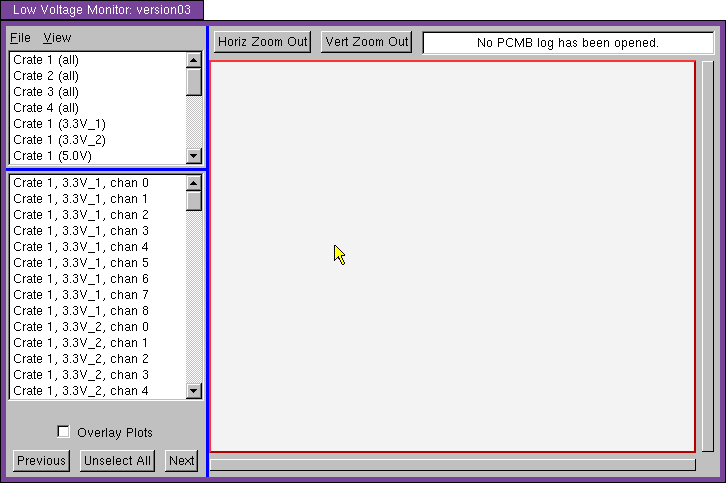
\includegraphics[width=0.9\linewidth]{01.png}
\end{center}
\end{frame}

\begin{frame}
\frametitle{Opening a file}
\begin{center}
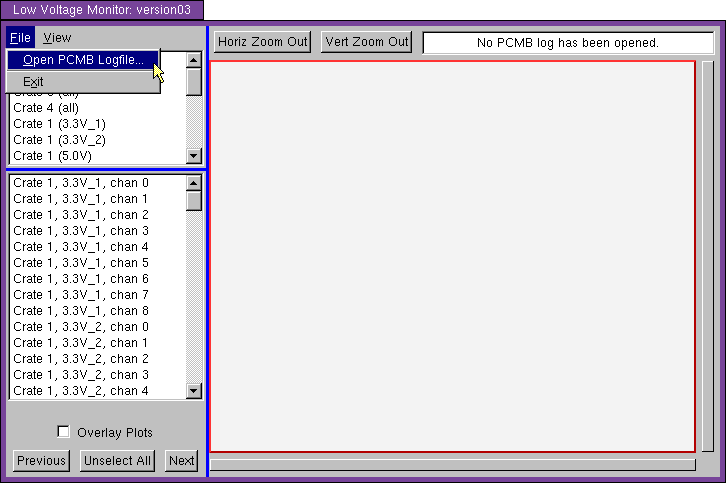
\includegraphics[width=0.9\linewidth]{02.png}
\end{center}
\end{frame}

\begin{frame}
\frametitle{PCMB only for now}
\begin{center}
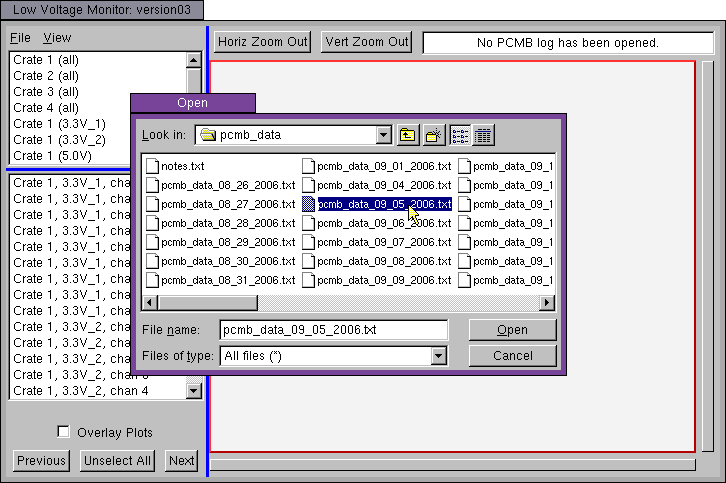
\includegraphics[width=0.9\linewidth]{03.png}
\end{center}
\end{frame}

\begin{frame}
\frametitle{Select 3.3~V channel 5}
\begin{center}
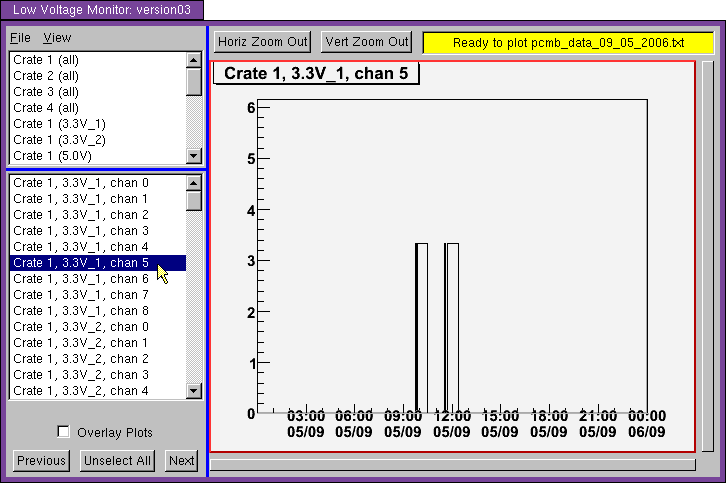
\includegraphics[width=0.9\linewidth]{04.png}
\end{center}
\end{frame}

\begin{frame}
\frametitle{Change the horizontal zoom (bottom scrollbar)}
\begin{center}
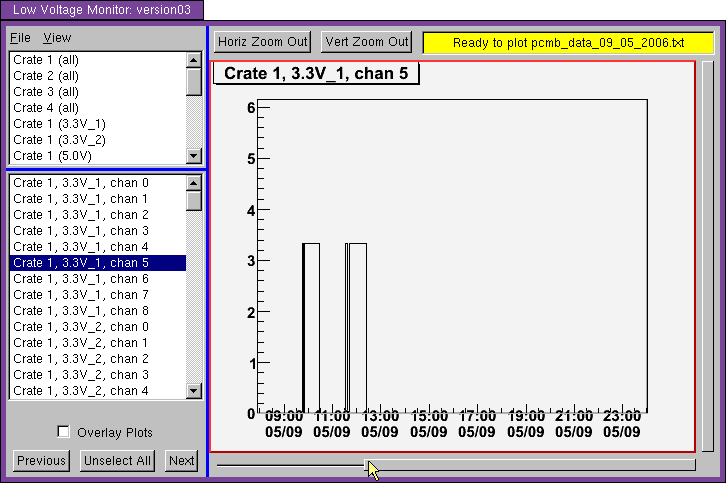
\includegraphics[width=0.9\linewidth]{05.png}
\end{center}
\end{frame}

\begin{frame}
\frametitle{Change the horizontal zoom (bottom scrollbar)}
\begin{center}
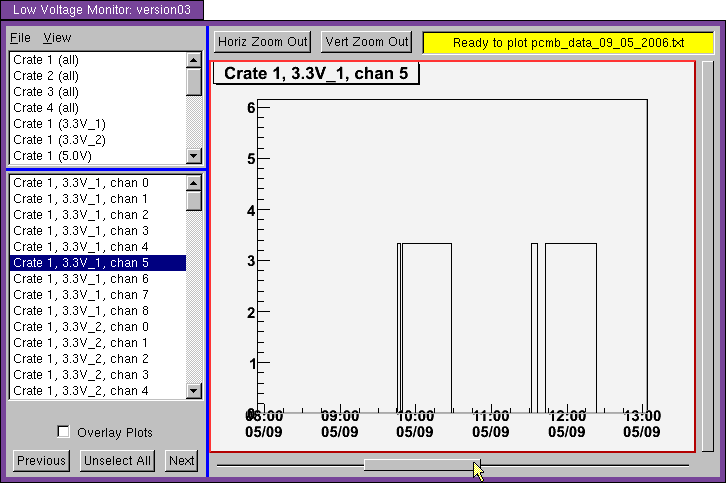
\includegraphics[width=0.9\linewidth]{06.png}
\end{center}
\end{frame}

\begin{frame}
\frametitle{Select all channels in crate 1}
\begin{center}
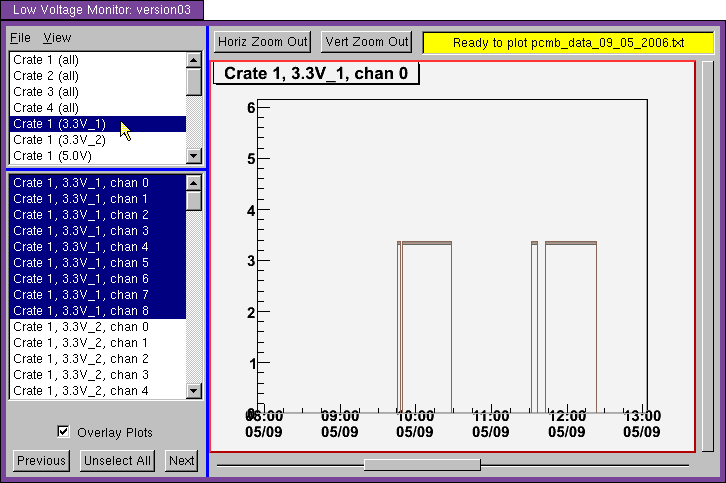
\includegraphics[width=0.9\linewidth]{07.png}
\end{center}
\end{frame}

\begin{frame}
\frametitle{Change the vertical zoom (right scrollbar)}
\begin{center}
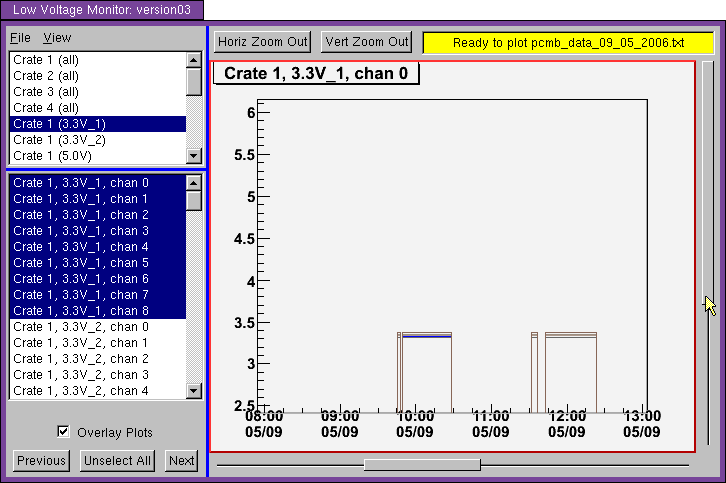
\includegraphics[width=0.9\linewidth]{08.png}
\end{center}
\end{frame}

\begin{frame}
\frametitle{Change the vertical zoom (right scrollbar)}
\begin{center}
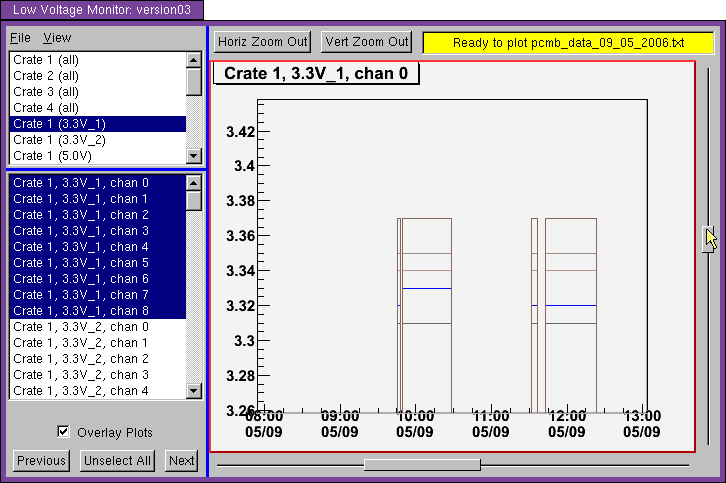
\includegraphics[width=0.9\linewidth]{09.png}
\end{center}
\end{frame}

\begin{frame}
\frametitle{Turn off one channel (the blue one)}
\begin{center}
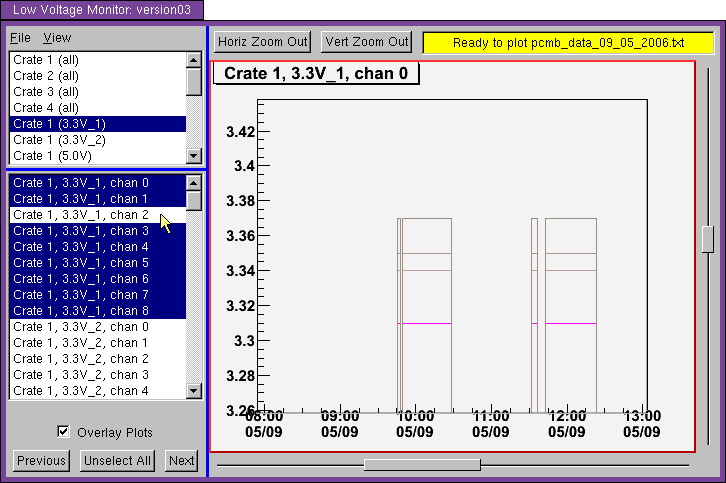
\includegraphics[width=0.9\linewidth]{10.png}
\end{center}
\end{frame}

\begin{frame}
\frametitle{Turn off plot overlay}
\begin{center}
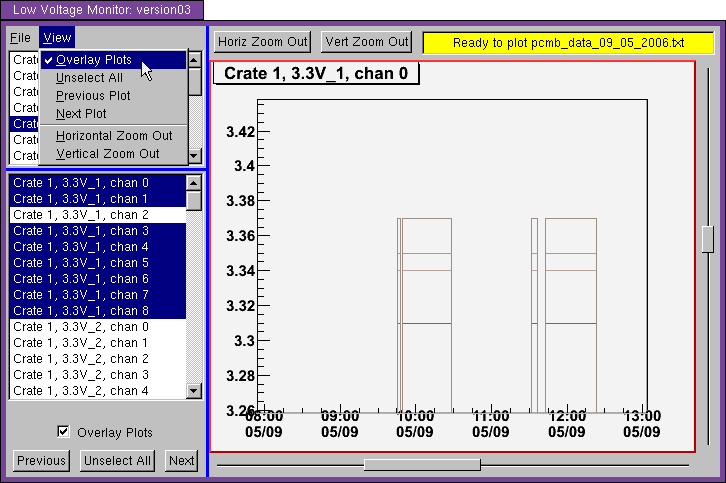
\includegraphics[width=0.9\linewidth]{11.png}
\end{center}
\end{frame}

\begin{frame}
\frametitle{Next}
\begin{center}
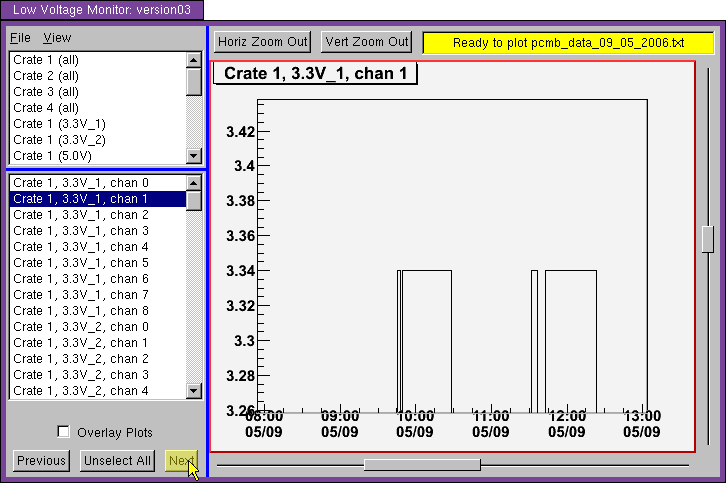
\includegraphics[width=0.9\linewidth]{13.png}
\end{center}
\end{frame}

\begin{frame}
\frametitle{Next}
\begin{center}
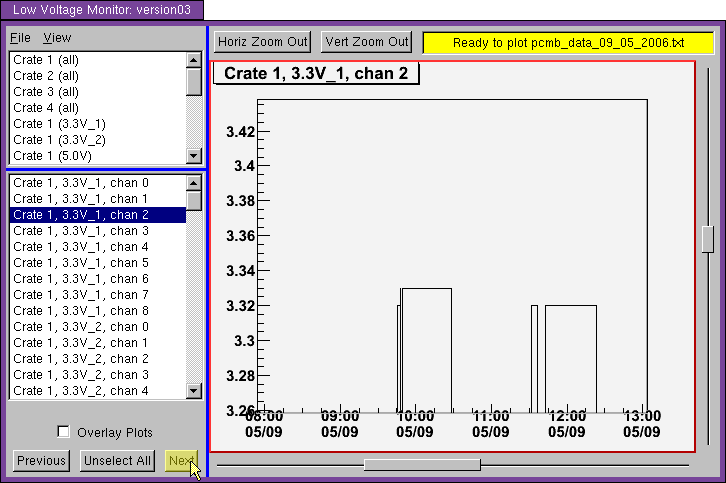
\includegraphics[width=0.9\linewidth]{14.png}
\end{center}
\end{frame}

\begin{frame}
\frametitle{Next}
\begin{center}
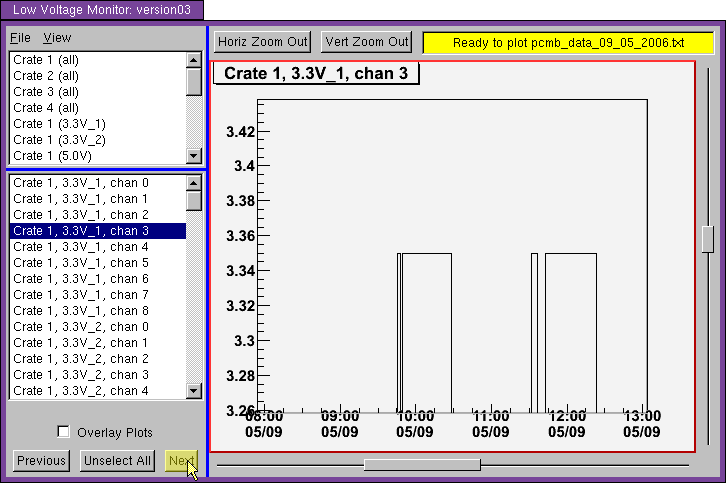
\includegraphics[width=0.9\linewidth]{15.png}
\end{center}
\end{frame}

\begin{frame}
\frametitle{Open multiple files}
\begin{center}
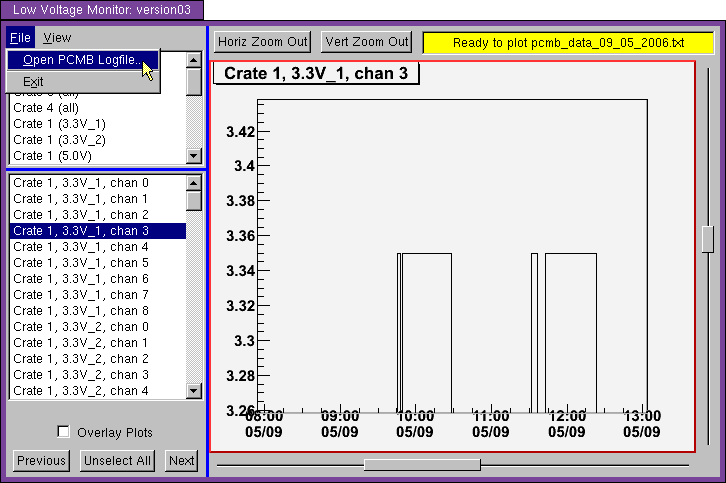
\includegraphics[width=0.9\linewidth]{16.png}
\end{center}
\end{frame}

\begin{frame}
\frametitle{Select next day}
\begin{center}
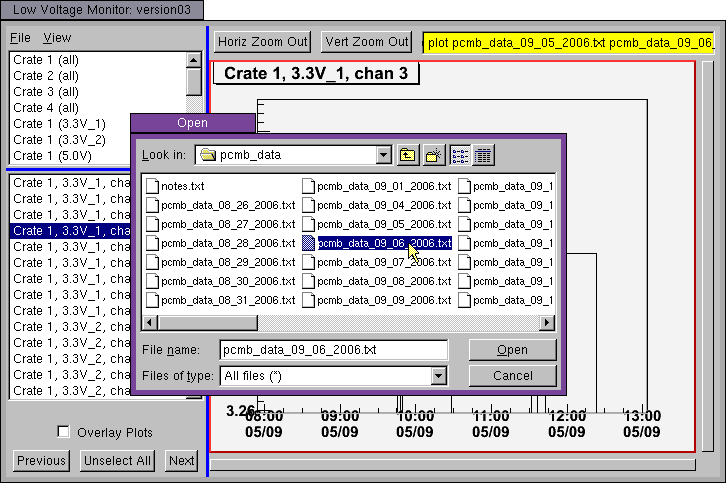
\includegraphics[width=0.9\linewidth]{17.png}
\end{center}
\end{frame}

\begin{frame}
\frametitle{Horiz zoom out to see both days (with separator)}
\begin{center}
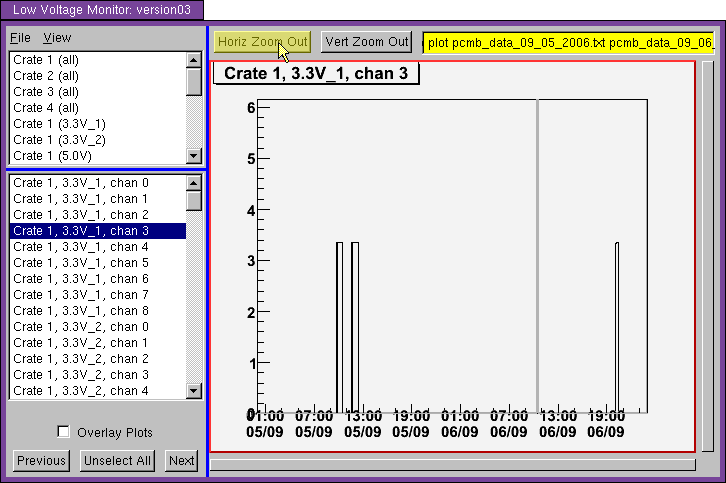
\includegraphics[width=0.9\linewidth]{18.png}
\end{center}
\label{numpages}
\end{frame}

\end{document}
